% !TeX root = ../praktikum.tex
% !TeX encoding = UTF-8
% !Tex spellcheck = de_DE

\subsection{Zweidimensionales Elektronengas}

Damit es zum Quanten-Hall-Effekt kommen kann, müssen einige Bedingungen erfüllt sein. Eine davon ist die Existenz eines zweidimensionalen Elektronengases.
In einem zweidimensionalen Elektronengas (2DEG) ist die Bewegung der freien Elektronen auf eine Ebene eingeschränkt. Es gibt verschiedene Möglichkeiten dies zu erreichen. 
\subsubsection{Aufbau der Probe}
In diesem Versuch wird dazu eine AlGaAs-GaAs-Heterostruktur verwendet, siehe Abbildung \ref{fig:Proben_Aufbau}. Die darin gestapelten, unterschiedlichen, einkristallinen Halbleitermaterialien sorgen aufgrund ihrer verschiedenen Bandlücken dafür, dass der Verlauf der Leitungs- bzw. Valenzbandkante in Stapelrichtung einen sehr kleinen Potentialtopf für die Leitungsbandelektronen erzeugt. Der elektronische Transport ist so in Stapelrichtung stark eingeschränkt, während sich die Elektronen in den anderen beiden Raumrichtungen bewegen können. Dabei muss die Bandverbiegung so sein, dass der Bereich des Potentialtopfes nur wenige Nanometer zwischen den Schichten einnimmt.

\begin{figure}[h]
\centering
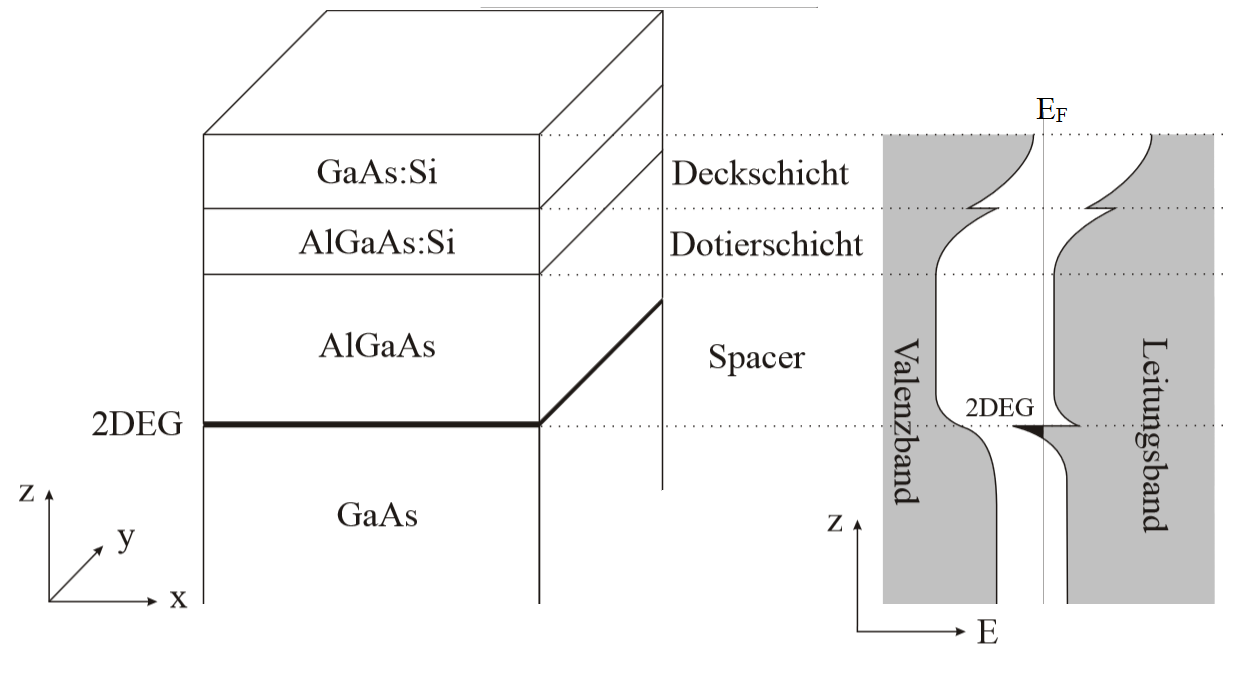
\includegraphics[width=0.7\linewidth]{images/Anleitungsheft/2DEG_Anleitungsheft}
\caption[2DEG Schicht]{vereinfachter Aufbau der GaAs-AlGaAs-Heterostruktur}
\label{fig:Proben_Aufbau}
\end{figure}

In Abbildung \ref{fig:Proben_Aufbau} ist der schematische Aufbau der in diesem Experiment untersuchten Probe dargestellt. 
Während sich die Gitterkonstanten der beiden Materialen um weniger als ein Prozent unterscheiden, liegt die Bandlücke des  Silizium-dotierten GaAs  höher als die des GaAs, sodass das Leitungsband des GaAs energetisch günstigere Zustände besitzt. Daher kommt es zum Elektronenfluss aus dem AlGaAs in das undotierte GaAs und so zu einem Verbiegen des Leitungs- und Valenzbandes, dargestellt in Abbildung \ref{fig:Proben_Aufbau}, rechts.
Der näherungsweise Potentialtopf, welcher sich im Leitungsband zwischen dem AlGaAs und dem GaAs ausbildet, besitzt ein Minimum unterhalb der Fermienergie $E_F$ und aufgrund seiner energetisch günstigeren Lage, werden die Elektronen in diesem Potentialtopf gefangen. 
In der Abbildung wird das AlGaAs auch als Spacer bezeichnet, denn diese Schicht in der Probe dient hauptsächlich dazu, Streupotentiale zwischen GaAs und der Dotierschicht AlGaAs:Si zu reduzieren, um die mittlere freie Weglänge und damit die Beweglichkeit der Elektronen zu erhöhen. Die Deckschicht GaAs:Si dient lediglich zum Schutz der Probe vor Oxidation und hat keine technische Bedeutung.

\subsubsection{Quantenmechanische Beschreibung unter Einfluss eines Magnetfeldes}
In der quantenmechanischen Beschreibung des 2DEGs findet man für die Energien der Elektronen aufgrund der Einschränkung ihrer Bewegung in z-Richtung quantisierte Werte. $E_z$ nimmt die Werte i mit i = 1, 2, 3, ... an, während die Bewegung der Elektronen in x- und y-Richtung uneingeschränkt bleibt.So setzt sich die Energie der Elektronen wie folgt zusammen:

\begin{equation}
E(k_x,k_y,i)=\frac{\hbar^2k_x^2}{2m^*}+\frac{\hbar^2k_y^2}{2m^*}+E_i^z   \text{~~~~~~~~~ mit ~~~} i=1,2,3....
\label{eq:energie_2DEG}
\end{equation}

Hier sind $k_x$ und $k_y$ die Wellenvektoren der Elektronen in $x -$ und $y-$ Richtung und $m^*$ ist die effektive Masse. $i = 1,2,3...$  entspricht der Quantisierung in $z-$ Richtung, welche zur Folge hat, dass sich für jedes Energieniveau ein zweidimensionales  Leitungsband in $x-$ und in $y-$ Richtung ausbildet. 
Es ist für das hier durchgeführte Experiment zum Quanten-Hall-Effekt essentiell, die Energierelationen der Elektronen im zweidimensionalen Elektronengas zu bestimmen. 

Die Zustandsdichte D in einem Band ergibt sich aus der Anzahl der Elektronenzustände $N$ pro Energieintervall und Probenvolumen $V$ und kann mit Gleichung~\eqref{eq:energie_2DEG} geschrieben werden als:

\begin{equation}
	D(E)=\frac{1}{V}\d{N(E)}{E}=g\frac{m^*}{2\pi\hbar^2}
	\label{eq:2DEG_zustandsdich} 
\end{equation}

Mit dem Probenvolumen V und der Teilchenzahl N. Der rechte Term folgt dabei aus der Zweidimensionalität des Probenvolumens und aus Gleichung \ref{eq:energie_2DEG}.
Die Zustandsdichte D(E) in dem Leitungsband eines 2DEGs ist also konstant mit dem Entartungsfaktor g. Für die Spinentartung ist $g_s=2$. Im senkrechten Magnetfeld ist die Bewegung der Elektronen auch in der xy-Ebene festgelegt.

Wenn nun ein Magnetfeld angelegt wird, werden die freien Elektronen klassisch durch die Lorentz-Kraft auf Kreisbahnen abgelenkt. Diese lässt sich durch die Überlagerung zweier senkrecht aufeinander stehenden harmonischen Schwingungen beschreiben, die senkrecht zueinander in der xy-Ebene schwingen. Der Abstand der Energiewerte ist durch $\hbar \omega_c$ gegeben,
mit der Kreisfrequenz:

\begin{equation}
\omega_c=\frac{eB}{m^*}
\label{eq:kreisfrequenz}
\end{equation}

Diese Kreisfrequenz wird auch Zyklotronfrequenz genannt. Da die Energieniveaus eines solchen Oszillators äquidistant sind, folgt für die Elektronenenergiedispersion des 2DEG in einem in z-Richtung angelegten Magnetfeld

\begin{equation}
E=E_i^z +(n+\frac{1}{2})\hbar\omega_c +g_L^*\mu_B Bs \text{~~~~~~~~~~mit~~~~~} n,i=1,2,3...
\label{eq:elektr_disp_bfeld}	
\end{equation}

Mit dem effektiven Lande-Faktor $g^*_L$, dem bohrschen Magneton $\mu_B$ und der Spinquantenzahl $s=\nicefrac{+}{-}\frac{1}{2}$.
Die Energien $E_n$ heißen Landau-Niveaus. Der mittlere Term der Gleichung beschreibt die kinetische Energie der Elektronen
in quantenmechanischer Betrachtung und der rechte Term berücksichtigt die Spin-Bahn-Wechselwirkung des Systems. 

\begin{figure}[h]
\centering
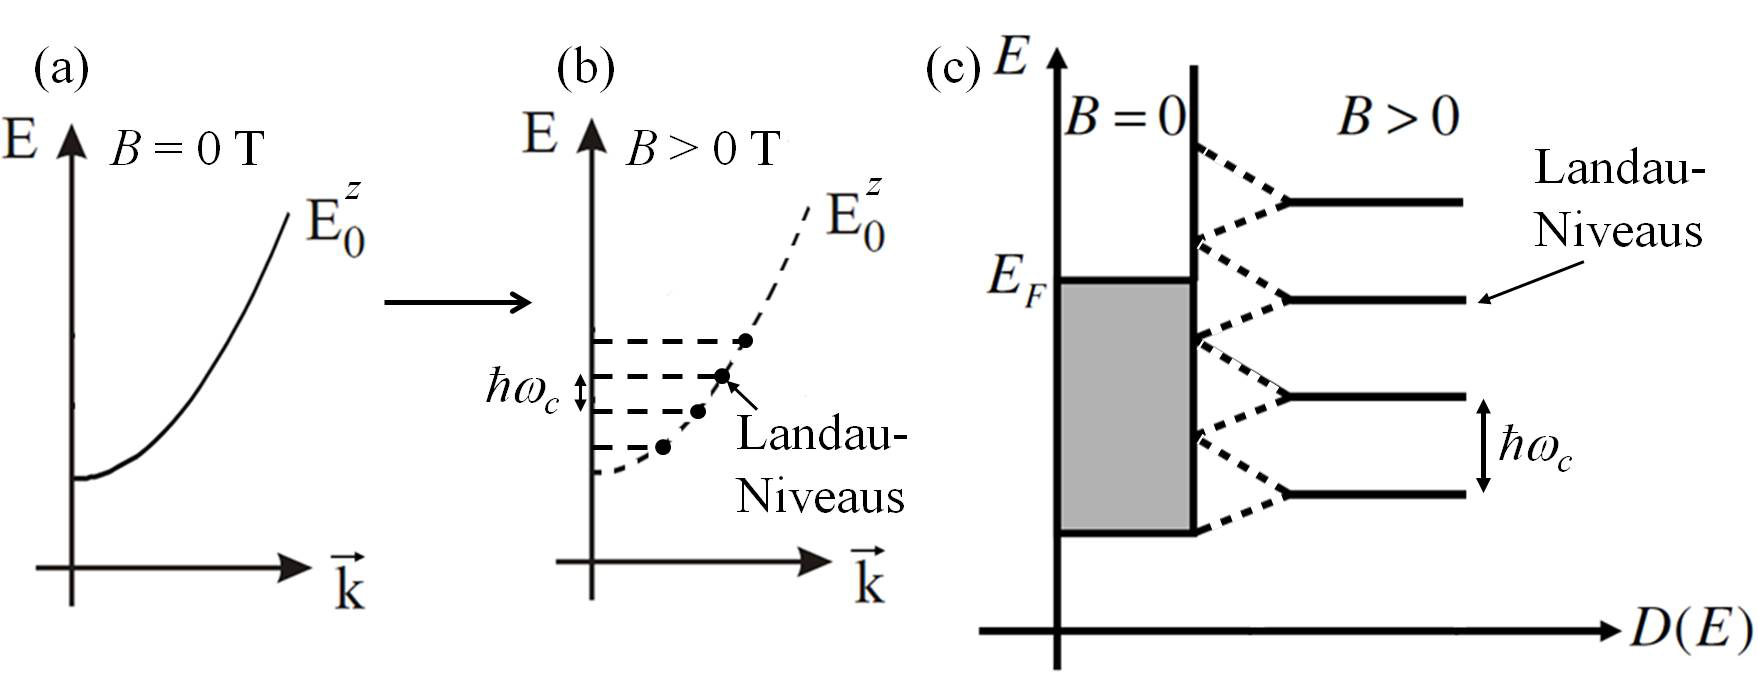
\includegraphics[width=0.7\linewidth]{images/Anleitungsheft/Landauniveaus_Anleitungsheft}
\caption[Landau Niveaus]{Vergleich der klassischen Beschreibung der Energieabhängigkeit (a) mit der Quantenmechanischen (b). (c) Vergleich des Zusammenhanges zwischen Zustandsdichte und Energie in klassischer und quantenmechanischer Beschreibung.}
\label{fig:Landauniveaus_Anleitungsheft}
\end{figure}

Abbildung \ref{fig:Landauniveaus_Anleitungsheft} veranschaulicht das Annehmen diskreter Werte der Zustandsdichte im quantenmechanischen Fall. 
Das Magnetfeld wirkt auf die Bewegungsrichtung der Elektronen, nicht aber auf deren kinetische Enegie, daher lässt sich die Anzahl der Elektronen pro Zustand mit der Zustandsdichte $D(E)$ bei $B=\unit[0]{T}$ ausdrücken mit

\begin{equation}
N_L=\frac{D(E)}{g}\hbar\omega_c = \frac{eB}{h}
\label{eq:zustandsd_pro_landauniveau}
\end{equation}

Daraus ist ersichtlich, dass die Anzahl der Elektronen pro Flächeneinheit, die ein Landauniveau aufnehmen kann, linear mit dem Magnetfeld zunimmt. Es wird ein Füllfaktor $\nu$ eingeführt, welcher angibt, wie viele Spin aufgespaltenen Landau-Niveaus bei gegebener Ladungsträgerdichte $n_s$ und einem Magnetfeld B zumindest teilweise besetzt sind:

\begin{equation}
\nu=\frac{n_s}{N_L}=\frac{hn_s}{eB}
\label{eq:einfuehrung_fuellfakt}
\end{equation}

\newpage
\subsection{Klassischer Hall-Effekt}

Beim klassischen Hall-Effekt liegt ein Magnetfeld B senkrecht zu einem stromdurchflossenen Leiter an. Das Magnetfeld wirkt durch die Lorentzkraft auf die bewegten Ladungsträger und es bildet sich die sogenannte Hallspannung $U_{Hall}$ senkrecht zur Strom- und Magnetfeldrichtung aus. Die Hallspannung ist proportional zum angelegten Magnetfeld. Dieser Effekt wurde 1879 von dem amerikanischen Physiker Edwin H. Hall entdeckt.

\begin{figure}[h]
	\centering
	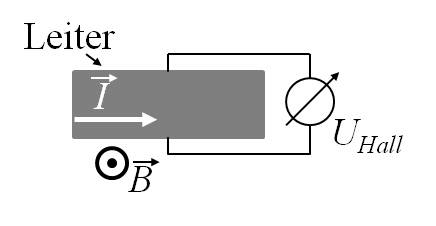
\includegraphics[width=0.4\linewidth]{images/Anleitungsheft/U_HALL_Anleitungsheft}
	\caption[Halleffekt klassisch]{Schematischer Aufbau zur Beobachtung des klassischen Hall-Effekts}
	\label{fig:U_HALL_Anleitungsheft}
\end{figure}

Für das in diesem Versuch verwendete 2DEG lässt sich die Beweglichkeit der Ladungsträger mit der Drude-Transporttheorie annähern. Diese basiert auf der Tatsache, dass sich die Bewegung der Ladungsträger im Elektronengas mit den klassischen Newtonschen Bewegungsgleichungen beschreiben lässt.
Man erhält die Bewegungsgleichung für Elektronen im E- und B-Feld im stationären Zustand:

\begin{equation}
\frac{m^*}{\tau} \vec{v}_D = -e(\vec{E}+\vec{v}_D \times \vec{B})
\label{eq:beweggl_stat}
\end{equation}

Mit $\tau$ als mittlere Stoßzeit zweier Elektronen und $\vec{v}_D$ als Driftgeschwindigkeit der Elektronen. Diese erhält man für $B=\unit[0]{T}$ aus:

\begin{equation}
\vec{v}_D=\frac{-e\tau}{m^*}\vec{E}=\mu\vec{E}
\label{eq:driftgeschw}
\end{equation}
mit der Beweglichkeit

\begin{equation}
\mu=\frac{-e\tau}{m^*}
\label{eq:bewegl_def}
\end{equation}

Die Stromdichte $\vec{j}$ beschreibt die Anzahl der Ladungen pro Zeit und Fläche und lässt sich anhand von Gleichung \ref{eq:driftgeschw} beschreiben durch:

\begin{equation}
\vec{j}=-en_s\vec{v}_D=en_s\mu\vec{E}=\sigma_0\vec{E}
\label{eq:stromdichte_herleitung}
\end{equation}
mit $\sigma_0$ als spezifischer Leitfähigkeit des Systems

\begin{equation}
\sigma_0=en_s\mu
\label{eq:sigma_def}
\end{equation}

Aufgrund der in z-Richtung eingeschränkten Elektronenbewegung innerhalb des 2DEGs, spielen nur die x- und y-Komponenten eine Rolle und Gleichung \ref{eq:stromdichte_herleitung} kann als Produkt aus Tensor und Vektor geschrieben werden

\begin{equation}
{j_x\choose j_y}=\begin{pmatrix}
\sigma_{xx} ~~ \sigma_{xy} \\ \sigma_{yx} ~~ \sigma_{yy}
\end{pmatrix} \cdot {E_x \choose E_y}
\label{eq:stromdichte_matrixdarst}
\end{equation}

Hierbei entsprechen die Einträge auf der Diagonalen des Tensors der spezifischen Leitfähigkeit in Richtung des elektrischen Feldes. Die Einträge auf der Nebendiagonalen sind nur für $B\neq0$ nicht Null.
Den spezifischen Widerstandstensor erhält man Matrixinversion.

\begin{equation}
\rho=\sigma^{-1}=\frac{1}{\sigma_{xx}\sigma_{yy} - \sigma_{xy}\sigma_{yx}}=\begin{pmatrix}
\sigma_{yy} ~~ \sigma_{xy} \\ \sigma_{yx} ~~ \sigma_{xx}
\end{pmatrix}
\label{eq:widerstandstensor_matrixinversion}
\end{equation}

Im hier durchgeführten Experiment wurde die Richtung des Stroms festgelegt und aus den gemessenen Daten zunächst die Komponenten des spezifischen Widerstandstensors $\vec{\rho}$ bestimmt. 
Diese erhält man aus

\begin{equation}
\rho_{xx}=\rho_{yy}=\frac{1}{e\mu n_s}
\label{eq:widerst_tensor_xx_yy}
\end{equation}
und
\begin{equation}
\rho_{xy}=-\rho_{yx}=\frac{1}{\mu n_s}B
\label{eq:widerst_tensor_xy_yx}
\end{equation}

Die Komponenten des Leitfähigkeitstensors ergeben sich über Matrixinversion aus dem Widerstandstensor, sodass spezifische Leitfähigkeit und spezifischer Widerstand gleichzeitig Null werden können. Man erhält über die Stromdichte $\vec{j}$ folgenden Zusammenhang von spezifischer Leitfähigkeit zu spezifischem Widerstand

\begin{align}
	\vec{j} = \sigma \cdot \vec{E} & & \Leftrightarrow & & \vec{E} = \rho \cdot \vec{j}
	\label{eq:e2rho}
\end{align}

bzw. 
\begin{equation}
\rho_{xx}=\frac{E_x}{j_X}
\label{eq:rho_xx_def}
\end{equation}
und 
\begin{equation}
\rho_{xy}=\frac{E_y}{j_X}
\label{eq:rho_xy_def}
\end{equation}

Zudem wurde im Experiment nicht die Stromdichte vorgegeben und das E-Feld gemessen, sondern es wurde die Spannung gemessen, indem der absolute Strom vorgegeben wurde. Die Probe entsprach hierzu der sogenannten Hall-Streifen-Geometrie. 

\begin{figure}
\centering
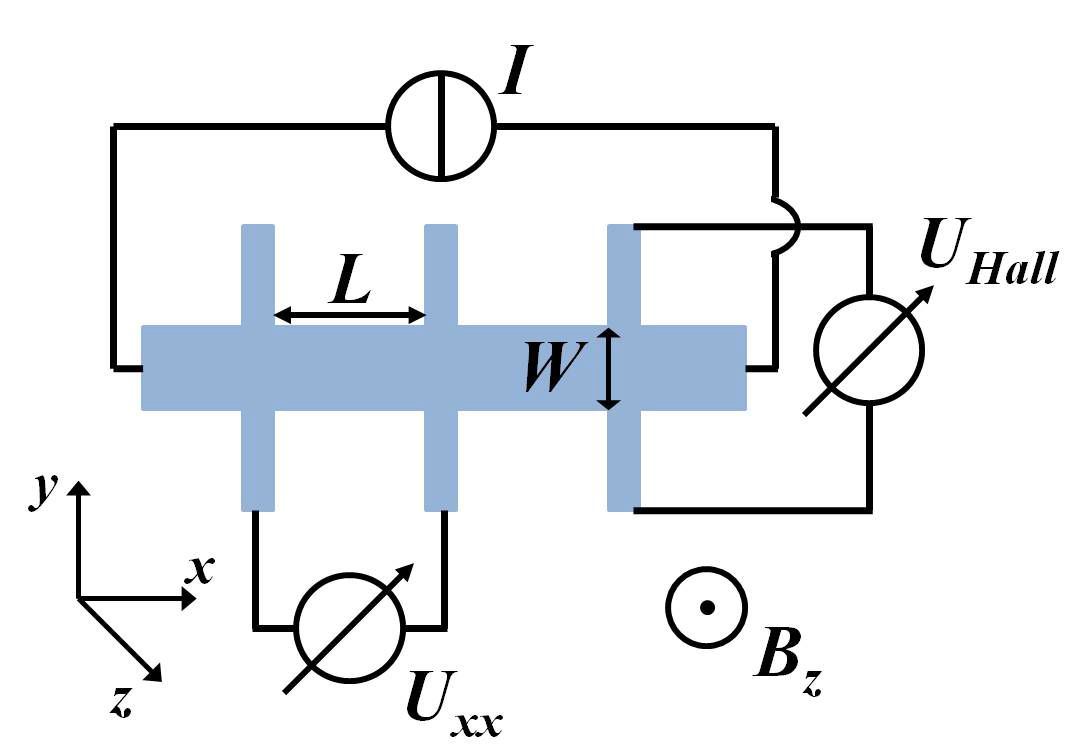
\includegraphics[width=0.4\linewidth]{images/Anleitungsheft/Hallstreifen_Geometrie_Anleitungsheft}
\caption[Hallstreifengeometrie]{schematische Darstellung der Hall-Streifen-Geometrie der Probe}
\label{fig:Hallstreifen_Geometrie_Anleitungsheft}
\end{figure}

Das hat den Vorteil, dass kein Strom durch die Kontakte fließt, an welchen die Hallspannung gemessen wird, sodass Kontaktwiderstände keine Rolle spielen, sondern nur die in der Probe abfallende Spannung. Der absolute Strom ist dann gegeben durch

\begin{equation}
I=j \cdot W
\label{eq:absoluter_Strom}
\end{equation}

Mit der Breite des Hallstreifens W. Die Längsspannung $U_{xx}$ ergibt sich aus

\begin{equation}
U_{xx}=E_x \cdot L
\label{eq:laengsspannung}
\end{equation}

Mit der Probenlänge L. Mit den Zusammenhängen aus Gleichung \ref{eq:rho_xx_def} und \ref{eq:rho_xy_def} ergibt sich für die spezifischen Widerstände

\begin{equation}
\rho_{xx}=\frac{U_{xx}}{I}\frac{W}{L}
\label{eq:rho_xx}
\end{equation}
und
\begin{equation}
\rho_{xy}=\frac{U_{Hall}}{I}
\label{eq:rho_xy}
\end{equation}

Daraus und aus den Gleichungen \ref{eq:widerst_tensor_xx_yy} und \ref{eq:widerst_tensor_xy_yx} folgt für die Ladungsträgerdichte im Leiter:
 
 \begin{equation}
 n_s=\frac{I}{e} \cdot \left( \d{U_{Hall}}{B} \right)^{-1}
 \label{eq:ladungsdichte_steig}
 \end{equation}
 Mit der Änderung der Hallspannung mit dem Magnetfeld $\d{U_{Hall}}{B}$. 
 
 Anhand der Ladungsträgerdichte und der in Stromrichtung über den Leiter abfallenden Spannung, kann man zudem die Beweglichkeit der Ladungsträger ermitteln:
 
 \begin{equation}
 \mu=\frac{1}{n_se}\frac{I}{U_{xx}}\frac{L}{W}
 \label{eq:bewegl_masse}
 \end{equation}

\newpage
\subsection{Quanten-Hall-Effekt und Shubnikov-de Haas-Oszillation}

Beim Quanten-Hall-Effekt bilden sich im Gegensatz zum klassischen Hall-Effekt waagerechte Plateaus für die Hallspannung aus. Diese sind materialunabhängig und ihre Werte sind durch Gleichung \ref{eq:qh_plateauwerte} gegeben. Die Plateaus bilden sich bei tiefen Temperaturen und bei Magnetfeldern ab einer Stärke von $|B| > \unit[2]{T}$ aus. Unterhalb dieser B-Feldstärke stimmen die Werte des quantenmechanischen Regimes in etwa mit dem des Klassischen überein. 

\begin{equation}
R_H=\frac{1}{\nu}\cdot 25812,8\Omega =\frac{1}{\nu} \frac{h}{e^2}
\label{eq:qh_plateauwerte}
\end{equation}

Dabei ist $\nu$ ein Füllfaktor, $h$ das Planksche Wirkungsquantum und e die Elementarladung. 

\begin{figure}[h]
\centering
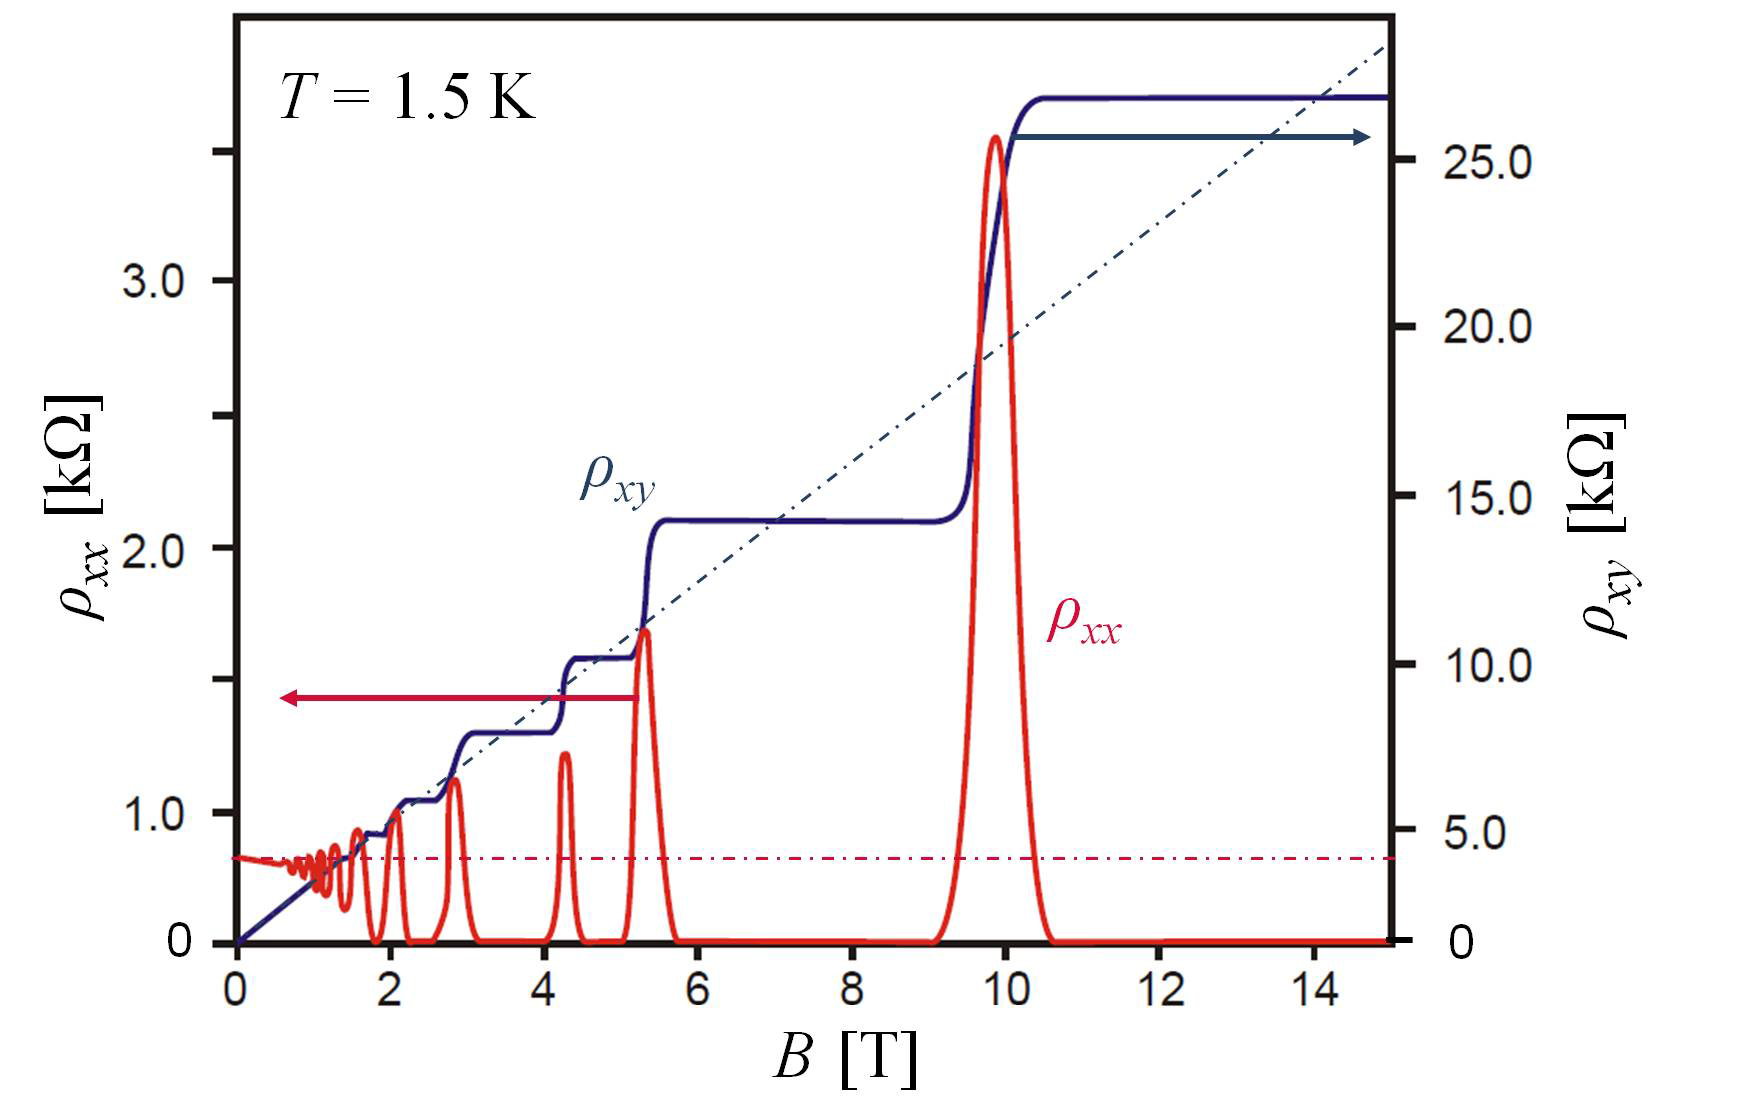
\includegraphics[width=0.5\linewidth]{images/Anleitungsheft/QH_Bsp_Messung_Anleitungsheft}
\caption[Bsp QH Oszill]{Beispielmessung des Quanten-Hall-Effekts und der Shubnikov-de Haas-Oszillation. Die gestrichelten Linien stellen die klassisch erwarteten Kurven dar. Es ist zu erkennen, dass sich spezifischer Längs- und Hallwiderstand bei kleinen Magnetfeldern verhalten wie klassisch zu erwarten. Mit steigendem B-Feld kommt es immer deutlicher zu Quanteneffekten. Der spezifsche Hall-Widerstand folgt dabei Werten mit ausgeprägten Plateaus, während im spezifschen Längswiderstand Shubnikov-de Haas-Oszillationen auftreten.}
\label{fig:QH_Bsp_Messung_Anleitungsheft}
\end{figure}

Während sich unter den Bedingungen des Quanten-Hall-Effekt für den Hallwiderstand die oben beschriebenen Plateaus ausbilden, sind für den spezifischen Längswiderstand der Probe Oszillationen zu beobachten. Man spricht von der sogenannten Shubnikov-de Haas-Oszillation. Bei einem sehr großen Magnetfeld nimmt der Längswiderstand im Minimum dieser Oszillation sogar den Wert Null an.

\subsubsection{Randkanalmodell}

Um die beiden hier betrachteten Effekte erklären zu können, wird das sogenannte Randkanalmodell verwendet. Dabei handelt es sich um eine Näherung, bei der am Rand der Probe ein Potential erzeugt wird, welches zu einer Erhöhung der Landau-Niveaus führt. Obwohl die Fermi-Energie $E_F$ im Inneren der Probe zwischen zwei Landau-Niveaus liegen, können so am Probenrand auch elektronische Zustände nahe der Fermi-Energie entstehen. Es bilden sich also eindimensionale Randkanäle zum Transport der Ladungsträger aus. Diese können sich nur in eine Richtung bewegen, welche von der Orientierung des Magnetfelds abhängt. Die chiralen Zustände sind durch Einwirken des Magnetfeldes über die Lorentzkraft auf geladene Teilchen recht stabil und Ladungsträger können dadurch trotz  eventueller Stöße mit Phononen wieder auf ihre Bahn finden. Dies ist in der folgenden Abbildung \ref{fig:Randkanalmodell_Anleitungsheft} dargestellt.

\begin{figure}[h]
\centering
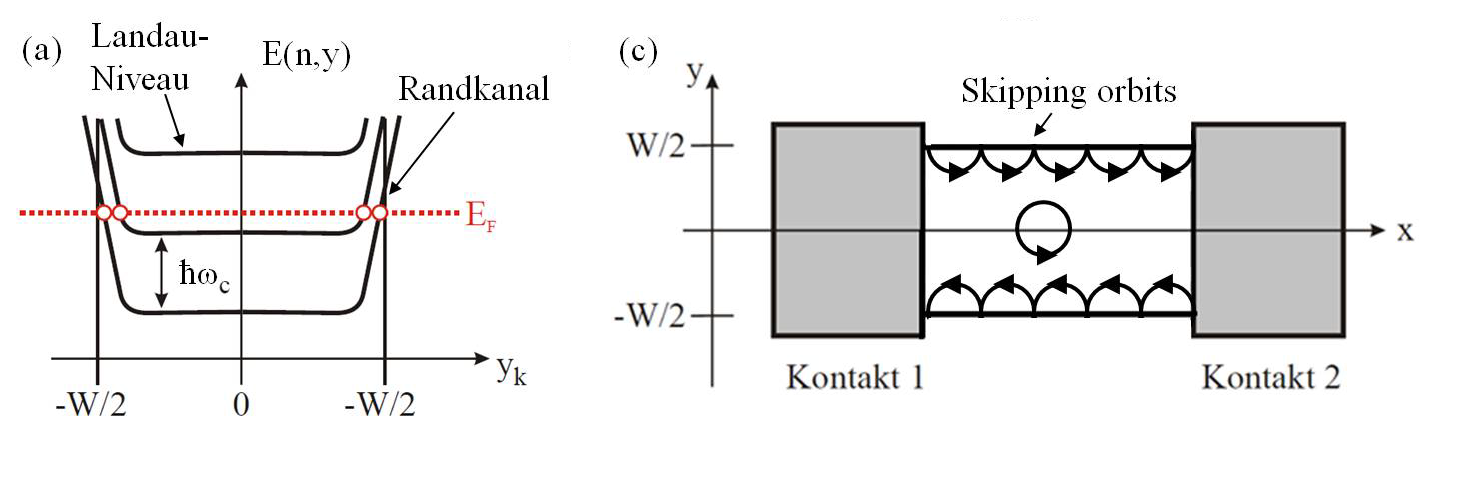
\includegraphics[width=0.7\linewidth]{images/Anleitungsheft/Randkanalmodell_Anleitungsheft}
\caption[Randkanalmodell]{\textbf{Links:} Schematische Darstellung der Erzeugung von Randpotentialen. \textbf{Rechts:} Schema zur Darstellung der Bewegung von Elektronen im Randkanalmodell}
\label{fig:Randkanalmodell_Anleitungsheft}
\end{figure}

Zur anschaulichen Beschreibung des Ladungstransport in den Randkanälen kann der Landauer-Büttiker-Formalismus genutzt werden. 
Dabei werden Parallelen von der Optik zur Technik aufgezeigt, wie zum Beispiel der Vergleich der Transmission einer Elektronenwelle mit der einer elektromagnetischen Lichtwelle. 

Die Anzahl M der Randkanäle hängt ab von der Lage der Fermienergie $E_F$ und somit auch von der Stärke des Magnetfeldes, wie in Abbildung \ref{fig:Randkanalmodell_Anleitungsheft} (a) dargestellt.
Die Hauptaussage des Landauer-Büttiker-Formalismus beruht auf der Annahme, dass die Elektronen mit einer Wahrscheinlichkeit $T_{lm}$ vom Kontakt m zum Kontakt l transmittiert werden. Dabei sei nun die Anzahl der Kontakte an der Probe $p=2$, diese liegen auf unterschiedlichen chemischen Potentialen $\mu_p$. Dann sei weiter am oberen Rand der Probe $T_{12}=1$ und $T_{21}=0$, denn ein Elektron, welches an Kontakt 1 in den Randkanal transmittiert wird, kann die Probe nur über Kanal 2 wieder verlassen. Am unteren Rand der Probe drehen sich die Wahrscheinlichkeiten genau um.  
Die gemessene Spannung an den beiden Kontakten ist dann

\begin{equation}
U_{12}=U_1 - U_2= \frac{\mu_2-\mu_1}{e}
\label{eq:spannung_randkanal}
\end{equation}

Den entsprechenden Strom erhält man aus 

\begin{equation}
I_0=-e(\int^{\mu_1}_0T_{12}D(E)v(E)dE-\int^{\mu_2}_0T_{12}D(E)v(E)dE)
\label{eq:strom_randkanal}
\end{equation}

Mit der Transmissionswahrscheinlichkeit T, der Zustandsdichte D(E)
und der Gruppengeschwindigkeit v(E) mit $v(E)=\frac{1}{\hbar}\pd{E}{k}$.

Der gesamte Nettostrom setzt sich aus dem Strom des oberen und unteren Kanals zusammen und beträgt

\begin{equation}
I=I_0+I_u=-e\int^{\mu_1}_{\mu2}T_{12}D(E)v(E)dE=\frac{e^2}{h}(U_1-U_2)
\label{eq:randkanal_nettostrom}
\end{equation}
 

\subsubsection{Erklärung der Hall-Plateaus und der SDH-Oszillation}

Randkanalmodell und Landauer-Büttiker-Formalismus (oben beschrieben) sind zwei Ansätze zur Erklärung der Ursache für die Hall-Plateaus und die Shubnikov-de Haas-Oszillation (SDH-Oszillation). 
Betrachtet wird nun eine Vierpunkt-Messung, wie sie in Abbildung \ref{fig:Vierpunktmessung_Anleitungsheft} dargestellt ist. 

\begin{figure}[h]
\centering
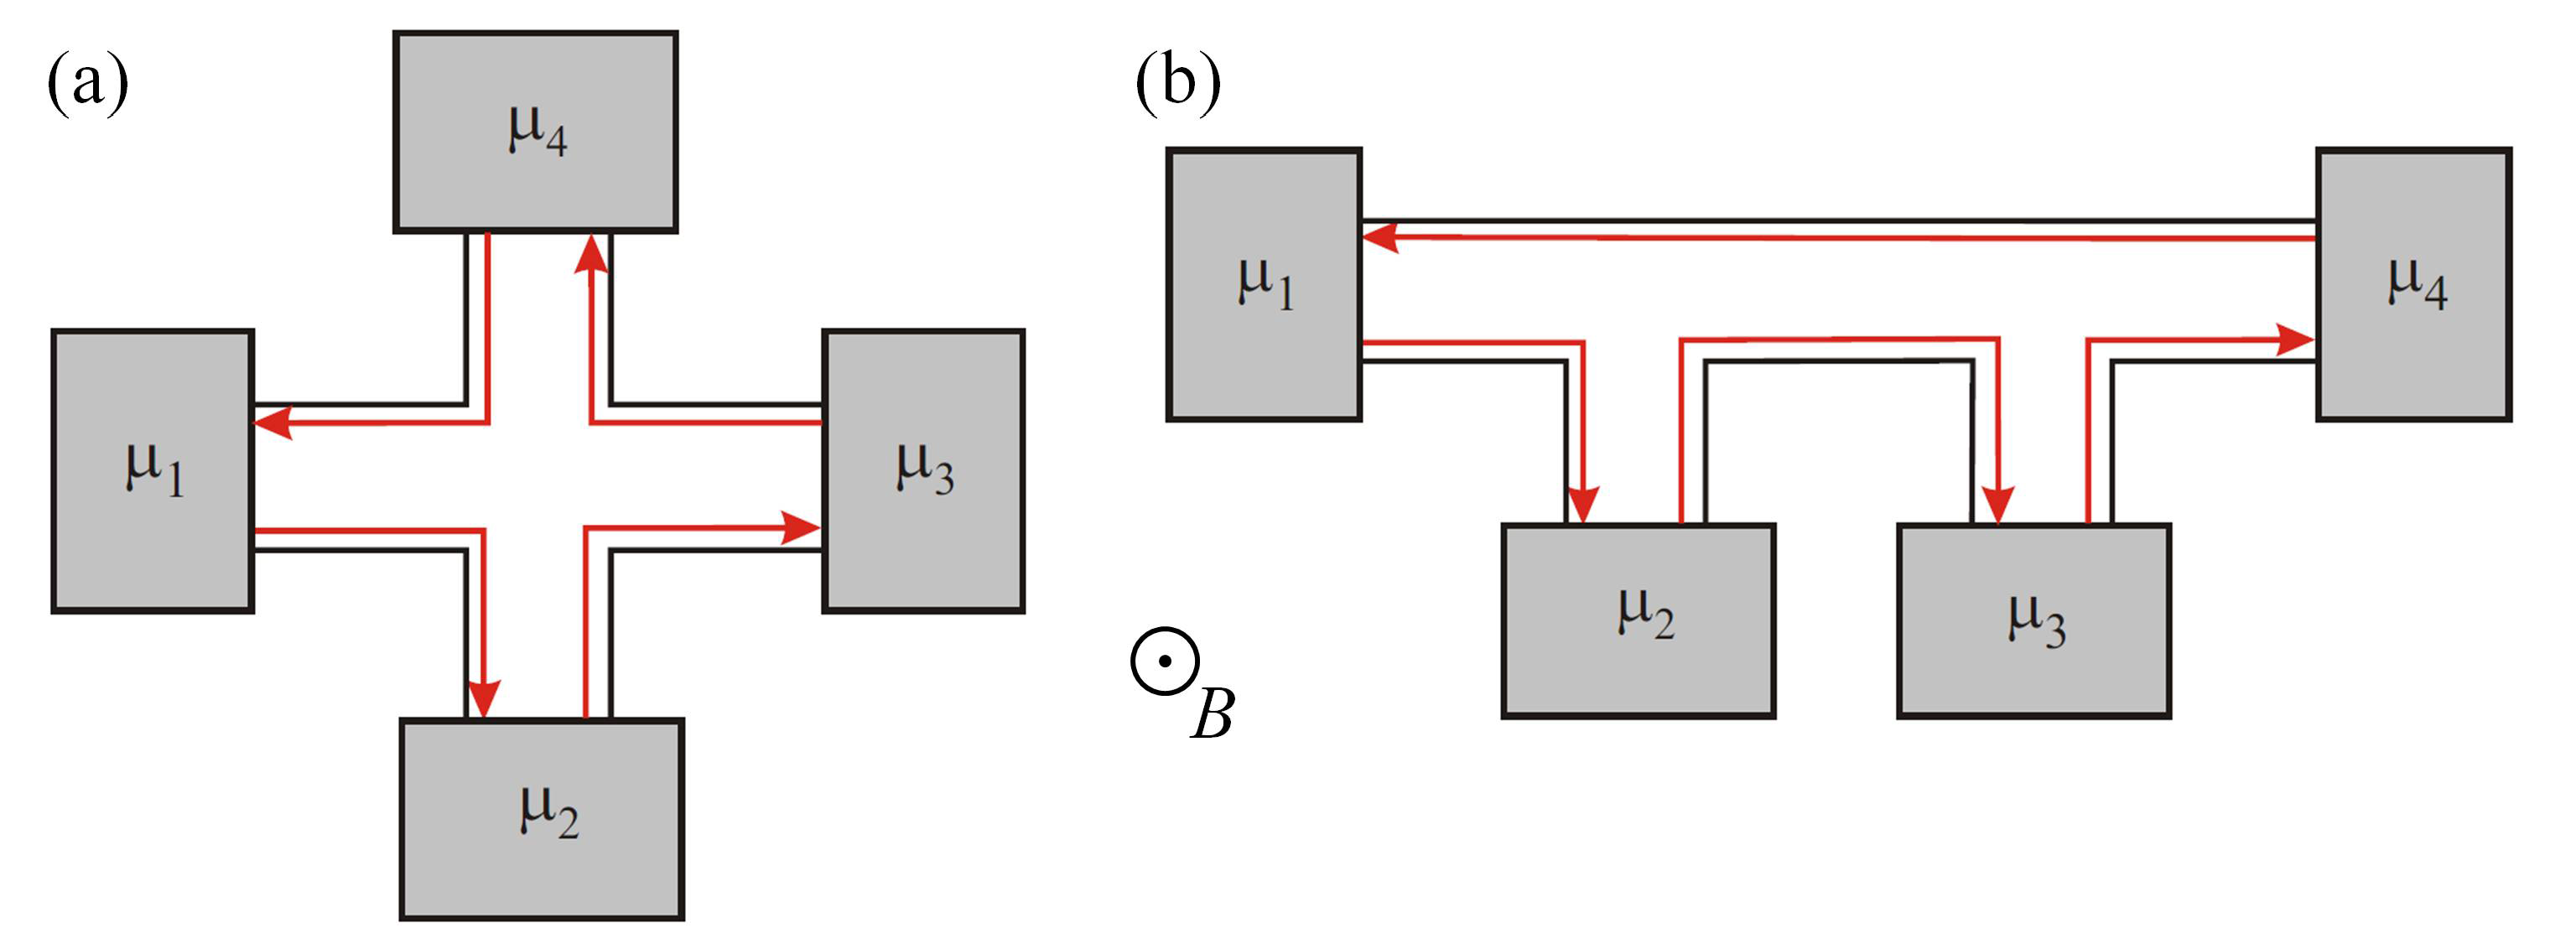
\includegraphics[width=0.7\linewidth]{images/Anleitungsheft/Vierpunktmessung_Anleitungsheft}
\caption[fig:vierpunktmessung]{\textbf{Links:} Schema der sogenannten Hall-Kreuz-Geometrie zur Messung der Hall-Spannung. \textbf{Rechts:} Schema der Kontaktgeometrie zur Messung des Längswiderstandes}
\label{fig:Vierpunktmessung_Anleitungsheft}
\end{figure}

Die roten Pfeile in der Abbildung \ref{fig:Vierpunktmessung_Anleitungsheft} zeigen die mögliche Richtung des Stromflusses in den Randzuständen an. Deren Anzahl sei M. Ströme, die in einen Kontakt hinein fließen, seien positiv. 
Anhand Gleichung \ref{eq:randkanal_nettostrom} lassen sich in diesem Beispiel die vier Ströme berechnen und man erhält ein Gleichungssystem dessen Lösungen die Hallspannung $U_{Hall}=U_4-U_2$ liefern. 
Mithilfe des Ohmschen Gesetzes erhält man den Hallwiderstand über

\begin{equation}
R_H=\frac{U_H}{I}=\frac{1}{M}\frac{h}{e^2}
\label{eq:U_Hall_simpel}
\end{equation}

Anhand dieser Formel ist zu erkennen, dass der Hallwiderstand also von der Anzahl der Randkanäle abhängt. Die Anzahl der Randkanäle änderst sich, wenn ein Landau-Niveau die Fermienergie durchläuft. dies geschieht in den Übergangsbereichen zwischen zwei Plateaus. Infolgedessen ändert sich also auch der Wert für die den Hallwiderstand $R_H$. Dies erklärt das Erscheinen der Plateauwerte im Hallwiderstand. Die Übergangsbereiche werden im Unterkapitel \ref{sec:lokalisierte Zust} näher erläutert. 
Es wird erneut der Landauer-Büttiker-Formalismus zur Hand genommen, um das Verschwinden des Längswiderstandes im Bereich eines Plateaus zu erklären. Im Bereich eines Plateaus liegt die Fermienergie zwischen zwei Landau-Niveaus und dadurch liegen die Kontakte über welche die Längsspannung gemessen wird, auf dem selben Potential. Das führt dazu, dass die Längsspannung den Wert Null annimmt. Für eine ideale Probe ist dies allerdings nur bei singulären Magnetfeldwerten tatsächlich der Fall.


\subsubsection{Lokalisierte Zustände}
\label{sec:lokalisierte Zust}

Die Fermienergie liegt per Definition zwischen dem höchsten besetzten und dem niedrigsten unbesetzten Elektronenniveau. Die Landau-Niveaus haben den Abstand $\hbar\omega_c$. Dieser wächst linear mit dem B-Feld. Das hat zur Folge, dass die teilweise gefüllten Landau-Niveaus zu größeren Energien hin verschoben werden und gleichzeitig entvölkert werden, da sich ihre relative Höhe zur Fermienergie verändert. Besitzt das Niveau unterhalb der Fermienergie einen ausreichend hohen Entartungsgrad, ist das oberhalb der Fermienergie liegende Niveau vollständig entvölkert und im Verhätnis fällt so die Fermi-Energie auf das nächst kleinere Energieniveau ab. Dies ist schematisch in Abbildung \ref{fig:Lokalisierte_Zust_Anleitungsheft} dargestellt.

\begin{figure}[h]
\centering
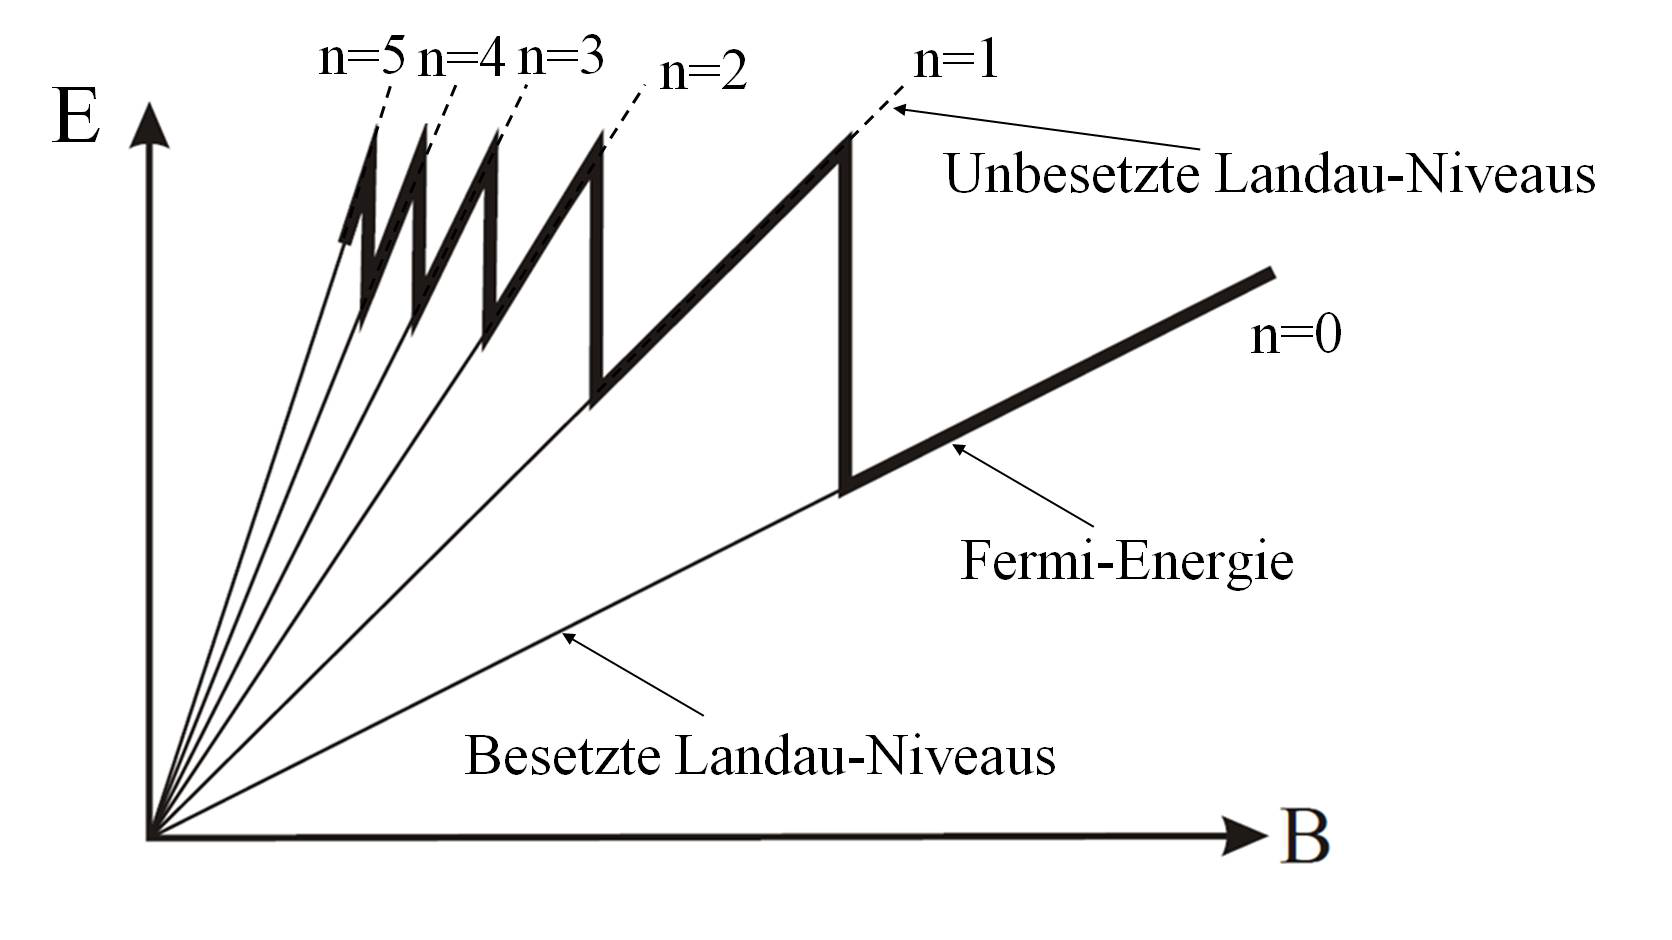
\includegraphics[width=0.7\linewidth]{images/Anleitungsheft/Lokalisierte_Zust_Anleitungsheft}
\caption[fig:landau vs fermi]{Abhängigkeit der Landau-Niveaus und der Fermi-Energie vom Magnetfeld}
\label{fig:Lokalisierte_Zust_Anleitungsheft}
\end{figure}

Eine ideale Probe zeichnet sich durch eine peak-förmige Zustandsdichte aus. Liegt ein singuläres Magnetfeld an, liegt die Fermienergie darin zwischen zwei Landau-Niveaus. Doch bei einer realen Probe treten Fluktuationen in der Zustandsdichte auf. Das liegt daran, dass die Landau-Niveaus im Inneren der Probe nicht konstant verlaufen, sondern durch Störstellen zu Verbreiterungen der Zustandsdichte führen.

\begin{figure}[h]
\centering
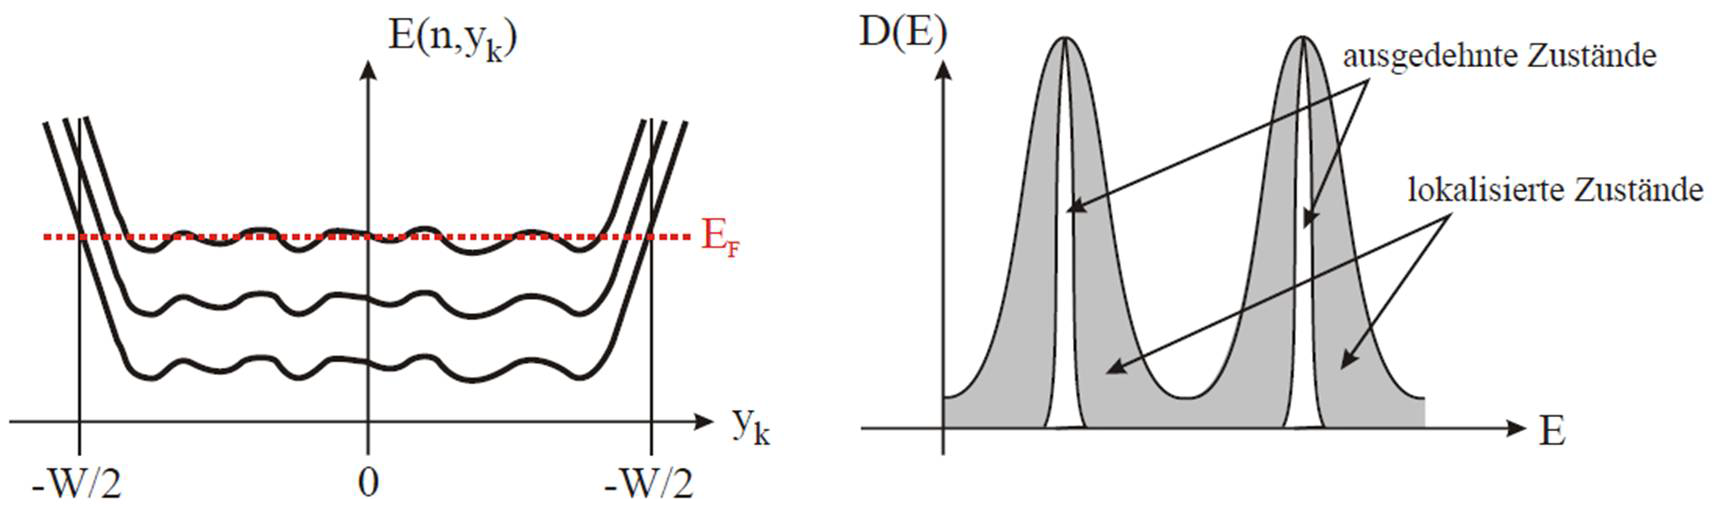
\includegraphics[width=0.7\linewidth]{images/Anleitungsheft/fermi_landau_Anleitungsheft}
\caption[fermi vs landau fig]{\textbf{Link:}Landau-Niveaus in einer realen Probe. \textbf{Rechts:} Verbreiterung der Zustandsdichte durch Störquellen}
\label{fig:fermi_landau_Anleitungsheft}
\end{figure}

Die chiralen Zustände des Randkanalmodells verschwinden in den Übergangsbereichen, in welchen die Fermienergie exakt auf einem LAndau-Niceau liegt. Dadurch kann es zu Rückstreuung kommen und der Längswiderstand ist nicht mehr Null.  
So lässt sich die Ursache der Ausdehnung der Hall-Plateaus, sowie die Minima der SDH-Oszillation mittels des Randkanalmodells zusammen mit dem Landauer-Büttiker-Formalismus und den lokalisierten Zuständen erklären.


\subsection{Plattenkondensator}

In der Auswertung des Versuchsteils zur Gatespannungsabhängigkeit wird näherungsweise von einem Plattenkondensator der Fläche A ausgegangen. Für die Anzahl der Ladungsträger gilt mit $N_s=n_s \cdot A$ 

\begin{equation}
N_s=C \cdot U_{Gate}
\label{eq:kondensator_ladung}
\end{equation}

mit der Kapazität C des Kondensators. Diese ist definiert über

\begin{equation}
C=\frac{\epsilon \epsilon_0 A}{d}
\label{eq:kondensator_abstand}
\end{equation}

mit dem Abstand d der Platten, der Dielektrizitätskonstanten des Vakuums $\epsilon_0$ und der Dielektrizitätskonstanten des Dielektrikums im Kondensator $\epsilon$. 
Aus \ref{eq:kondensator_ladung} und \ref{eq:kondensator_abstand} ergibt sich:
\begin{equation}
n_s=\frac{\epsilon \epsilon_0}{d}(U_{Gate}-U_{th})
\label{eq:kondens_lad_und_abst}
\end{equation}

mit der Einsatzspannung $U_{th}$.
